\section{Архітектура системи}
\subsection{Аудитована реалізація та межі компонентів}
Знімок системи --- коміт \code{f0e9d0d67422b0c286a2cb9e7d4e935a833a9533} від 9 листопада 2026 року в гілці \code{codex/social-master-plan-audit-remediation}. На момент аудиту локальна ревізія \code{main} була старішою й не містила відповідних виправлень. Перед створенням нових артефактів статті робоче дерево аудиту було чистим. Вихідний код, аналітичні скрипти, тести, схеми JSON, знімки даних, дослідницькі документи й звіти зберігаються в окремих каталогах. Наразі Social не розповсюджується як єдиний пакет і не має файла фіксації залежностей. Точками входу є модулі Python і дослідницькі скрипти, а не одна всеохопна команда застосунку.

На рисунку~\ref{fig:architecture} показано реалізовану будову. Збирачі платформ і попередня обробка для кейсу створюють знімки для застарілого аналізу інформації. Новіша типізована гілка пов'язує зібрані джерела з реєстром доказів та обмеженим аналізом. Індексування й обробка відео утворюють окремий локальний конвеєр; загальний запускач інциденту не викликає повний медіаконвеєр автоматично. Контролер інтегрує фіксований адаптер Source Watch і необов'язкові попередньо типізовані офлайн-входи. Він не запускає кожен збирач, не розширює пошук джерел автономно й не виводить кожен проміжний об'єкт із сирих записів.

\begin{figure}[!htbp]
\centering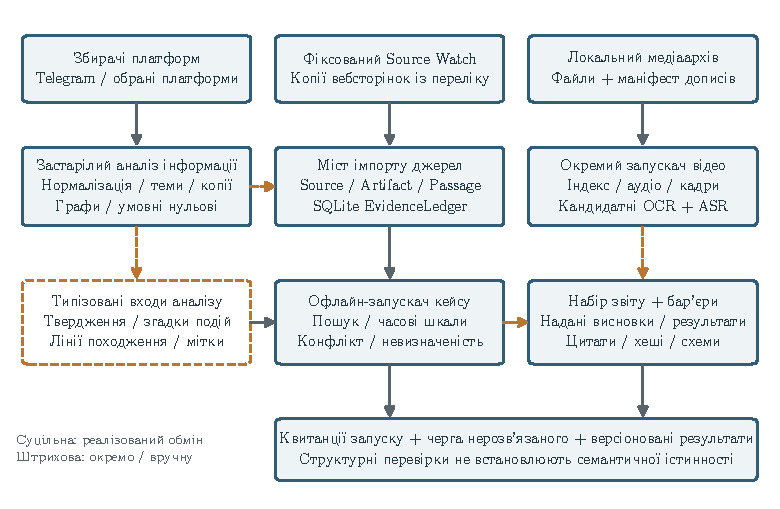
\includegraphics[width=\linewidth]{system_architecture.pdf}
\caption{Реалізовані компоненти Social та межі інтеграції на аудитованій ревізії. Суцільні стрілки позначають реалізований обмін; штрихові --- ручні або окремо запущені адаптери. Медійна й застаріла аналітична гілки виконувані, але загальний запускач інциденту оркеструє не всі з них.}
\label{fig:architecture}
\end{figure}

\begin{table}[!htbp]
\caption{Компоненти системи: реалізація й валідація є окремими вимірами. Шляхи вказано відносно кореня репозиторію; більшість аналітичних модулів розміщено в \code{src/analysis/}.}
\label{tab:components}\small
\begin{tabularx}{\linewidth}{@{}p{25mm}X p{25mm}@{}}\toprule
Компонент & Конкретна реалізація та роль & Свідчення готовності\\\midrule
Отримання даних & \code{src/tg_collect.py}, \code{src/tg_comments_collect.py}, \code{src/source_watch_collect.py}; окремі API- та вебзбирачі & Реалізовано; залежить від доступу, офлайн-тести\\
Підготовка знімків & \code{build_continuation.py}, \code{prep.py}; перевірене об'єднання й правила релевантності кейсу & Реалізовано; перевірки походження; семантична релевантність незалежно не валідована\\
Аналіз інформації & \code{analyze.py}, \code{coordination_lsh_audit.py}, \code{coordination_null_models.py} & Реалізовано; оцінено точний граф і обмежене повторне виконання\\
Облік доказів & \code{src/evidence_ledger.py}, \code{source_ingest_bridge.py}, \code{source_lineage.py} & Реалізовано; структурні тести й тести посилань\\
Оцінка доказів & \code{claim_verification.py}; BM25, евристики, агрегація & Пошук реалізовано; семантичні евристики експериментальні\\
Події та конфлікт & \code{event_reconstruction.py}, \code{conflict_analysis.py}; надані типізовані записи & Реалізовано впорядкування; фізичну істинність не оцінено\\
Локальні медіа & \code{src/media_pipeline.py}, \code{video_pipeline_runner.py}, \code{media_fingerprints.py} & Реалізовано; технічні квитанції; семантичні пороги не калібровані\\
Аналітика аудиторії & \code{audience_response.py}, \code{audience_aggregation.py} & Реалізовано контракти й агрегацію; мітки надані, точність не оцінено\\
Процес і звіти & \code{offline_case_runner.py}, \code{incident_orchestrator.py}, \code{report_generator.py}, \code{evaluation_harness.py} & Протестовано обмежену інтеграцію; наскрізне розслідування не валідоване\\\bottomrule
\end{tabularx}
\end{table}

Розрізнення в таблиці~\ref{tab:components} має операційне значення. Контрактні перевірки, вставлення в реєстр лише з додаванням і детерміновані процесори є повторно використовуваними механізмами. Переліки тверджень, обрані набори уривків, інтервали фізичних подій і еталонні рядки ASR в окремих збирачах є кураторськими дослідницькими входами. Скрипти досьє форматують результати; вони не перевіряють незалежно кожне емпіричне твердження, яке друкують. Схеми платформ можуть оголошувати платформу без наявного власного збирача. Жодну із цих категорій не слід зводити до твердження про готовність усього репозиторію до промислового використання.

\subsection{Зберігання та інтерфейси виконання}
Знімки JSON і JSONL забезпечують потокові записи й придатні для перегляду проміжні результати. CSV використовується для ребер графів, підсумків та окремих оцінювальних таблиць. SQLite зберігає зв'язані записи доказів. Сирі медіа й більші похідні зберігаються поза відстежуваними файлами коду, а маніфести пов'язують спостереження з байтами й похідним текстом. PDF і Markdown є формами подання, а не авторитетною заміною машинозчитуваних результатів.

Повторно використовуваний процес приймає \code{IncidentSpec}, явні типізовані входи, каталог результатів і ревізію Git виробника. Він фіксує поетапні квитанції та маніфест запуску. Викликач має надати справжню ревізію: запис рядка ревізії не доводить, що виконуваний код їй відповідав. Виконання обмежують бюджети, граничні часи, обмеження шляхів, обмежені розміри входів і явні стани \code{not_run}. Такий підхід віддає перевагу локальній придатності для перегляду й поступовому використанню на невеликій дослідницькій робочій станції, а не розподіленій агентній платформі, і залишає значну інтеграційну роботу на межі між збирачем і типізованим записом.
